\documentclass{beamer}
\usepackage{fancyvrb}

\usecolortheme{rose}
\usefonttheme{structurebold}
\setbeamercovered{again covered=\opaqueness<1->{50}}

\title[hsms]{Introduction to Hardware Security Modules}
\author{Joseph Birr-Pixton\\
@jpixton\\
http://jbp.io/}
\date{}

\begin{document}

\frame{\titlepage}

\frame
{
  \frametitle{Contents}

  \begin{enumerate}
    \item<1> Intro.
  \end{enumerate}
}

\frame
{
  \frametitle{Introduction}
  Who the hell am I?

  \begin{enumerate}
    \item<2->{Wrote software and firmware for nCipher 2005-2012.}
    \item<3->{nCipher acquired by Thales 2008.}
  \end{enumerate}
}

\frame
{
  \frametitle{WTF is an HSM?}

  \uncover<2->{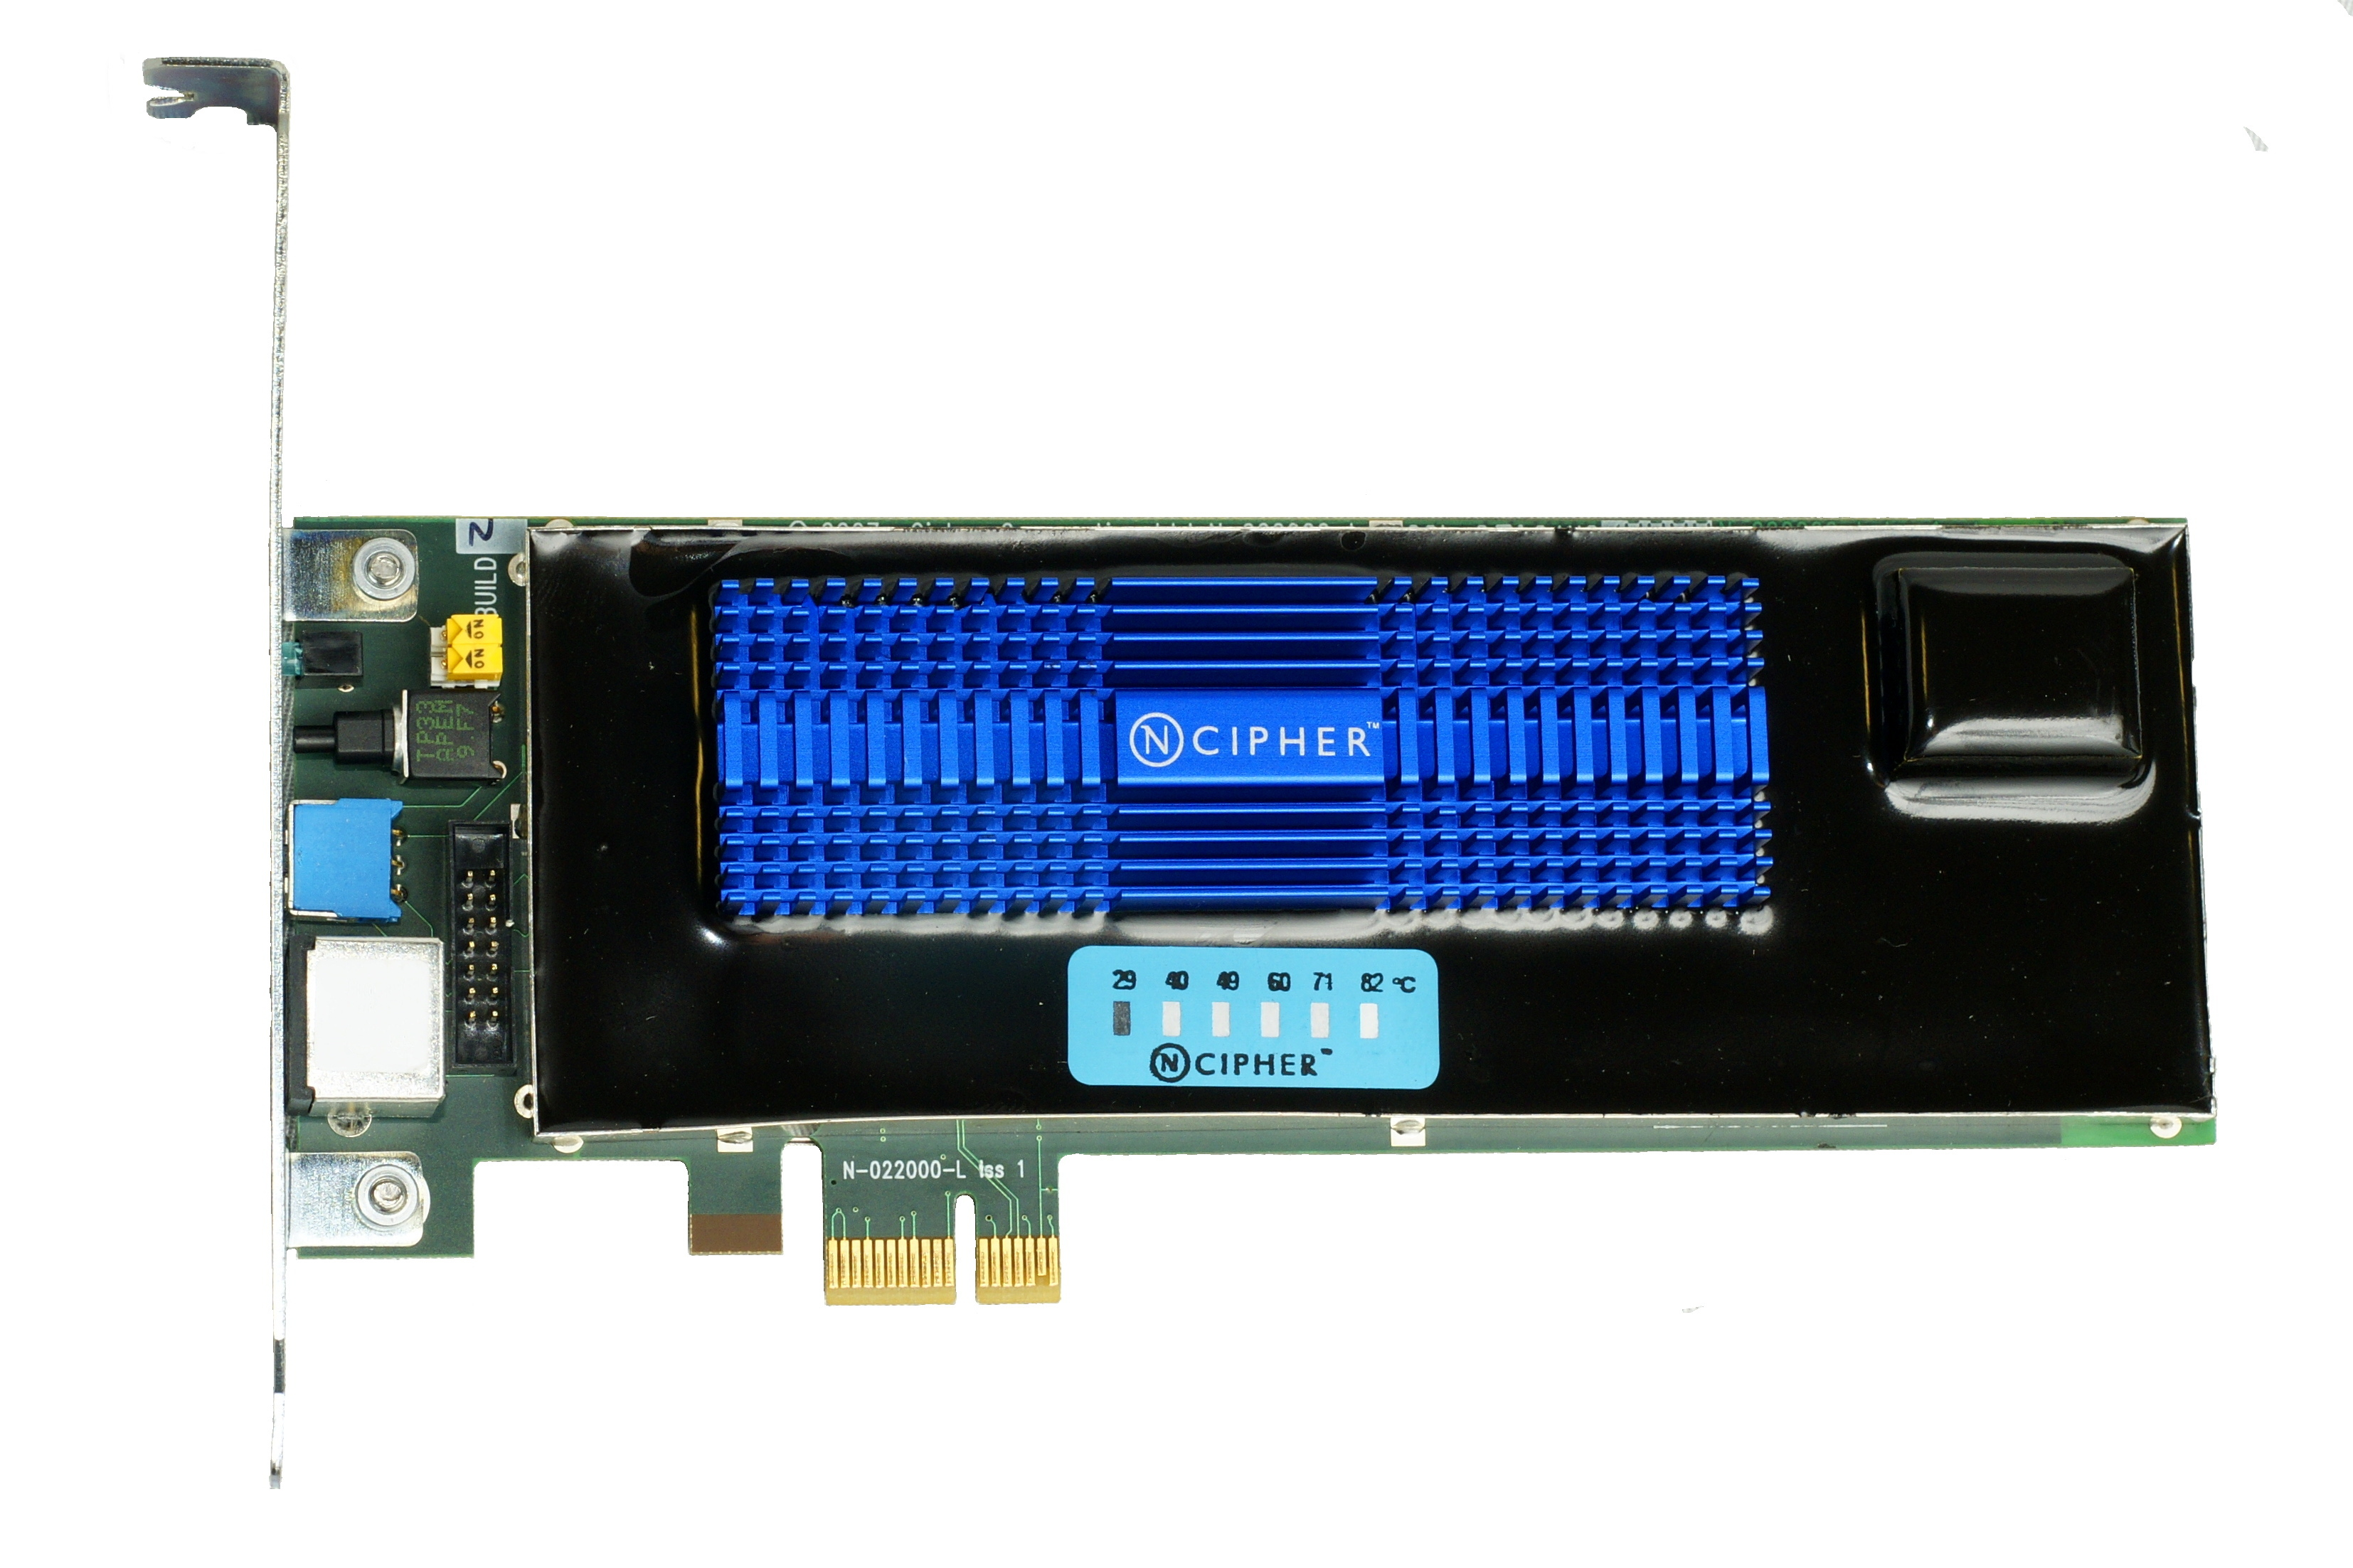
\includegraphics[width=1.0\textwidth]{imgs/NCipher_nShield_F3_Hardware_Security_Module.jpg}}
}

\frame
{
  \frametitle{WTF is an HSM?}

  \begin{itemize}
  \item<1-> Usually built from general purpose CPU, RAM, non-volatile storage.
  \item<2-> Often with a commercial or custom crypto accelerator.
  \item<3-> Some communications path to talk to the thing (PCI, PCIe, ethernet, USB, etc.)
  \item<4-> Hardware typically has physical protection:
    \begin{itemize}
    \item<5-> \emph{Tamper evident} hardware usually potted in epoxy-based compound.
    \item<6-> \emph{Tamper reactive} hardware usually enclosed in tamper sensing membrane, with active response circuitry within.
    \end{itemize}
  \end{itemize}
}

\frame
{
  \frametitle{Fin}
  Questions?
}

\end{document}
